\documentclass[tikz]{standalone}
\usepackage{pgfplots}
\pgfplotsset{compat=1.18}

% Define colors extracted from the image
\definecolor{matlabblue}{RGB}{0,114,189}
\definecolor{matlaborange}{RGB}{217,83,25}

\begin{document}
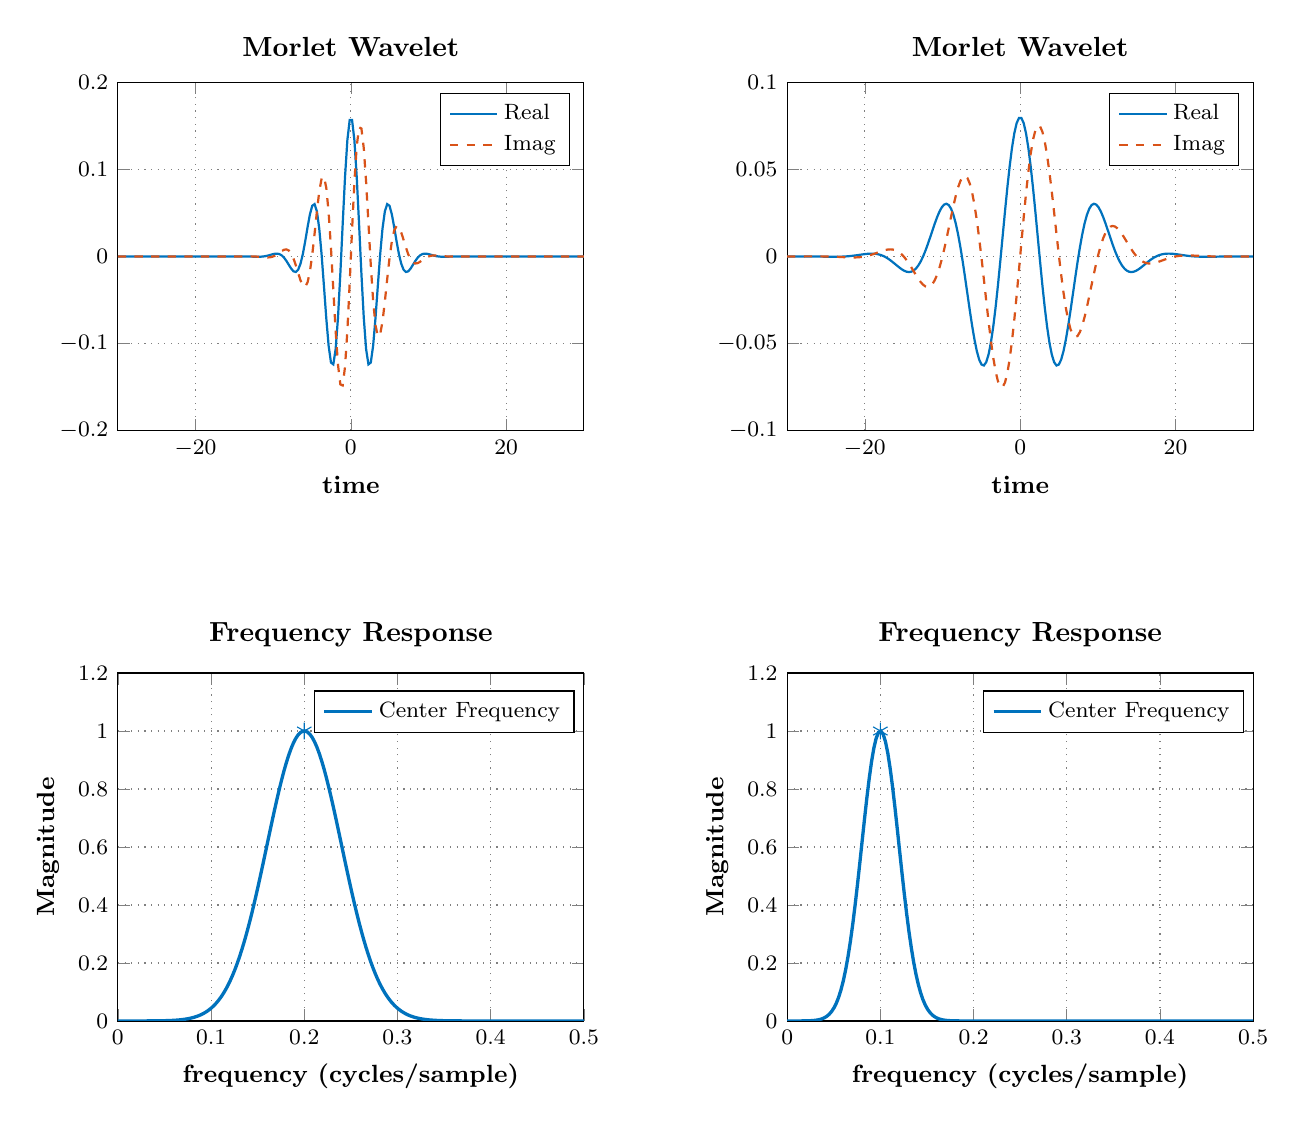
\begin{tikzpicture}
    % Common style for all plots to ensure consistency
    \pgfplotsset{
        every axis/.style={
            label style={font=\bfseries\small},
            title style={font=\bfseries},
            tick label style={font=\footnotesize},
            grid=major,
            major grid style={dotted, gray},
            width=7.5cm,
            height=6cm,
            legend style={font=\footnotesize, draw=black, fill=white, cells={anchor=west}}
        }
    }

    % --- Top Left: Morlet Wavelet (Time Domain, Scale 1) ---
    \begin{axis}[
        at={(0,0)},
        title={Morlet Wavelet},
        xlabel={time},
        xmin=-30, xmax=30,
        ymin=-0.2, ymax=0.2,
        ytick={-0.2,-0.1,0,0.1,0.2},
        legend pos=north east
    ]
        % Real part (Blue Solid)
        \addplot[matlabblue, thick, domain=-30:30, samples=200] 
            {0.16 * exp(-x^2/(2*3.5^2)) * cos(deg(2*pi*0.2*x))};
        \addlegendentry{Real}
        
        % Imaginary part (Orange Dashed)
        \addplot[matlaborange, thick, dashed, domain=-30:30, samples=200] 
            {0.16 * exp(-x^2/(2*3.5^2)) * sin(deg(2*pi*0.2*x))};
        \addlegendentry{Imag}
    \end{axis}

    % --- Top Right: Morlet Wavelet (Time Domain, Scale 2) ---
    \begin{axis}[
        at={(8.5cm,0)},
        title={Morlet Wavelet},
        xlabel={time},
        xmin=-30, xmax=30,
        ymin=-0.1, ymax=0.1,
        ytick={-0.1,-0.05,0,0.05,0.1},
        yticklabel style={/pgf/number format/fixed, /pgf/number format/precision=2},
        legend pos=north east
    ]
        % Real part
        \addplot[matlabblue, thick, domain=-30:30, samples=200] 
            {0.08 * exp(-x^2/(2*7^2)) * cos(deg(2*pi*0.1*x))};
        \addlegendentry{Real}
        
        % Imaginary part
        \addplot[matlaborange, thick, dashed, domain=-30:30, samples=200] 
            {0.08 * exp(-x^2/(2*7^2)) * sin(deg(2*pi*0.1*x))};
        \addlegendentry{Imag}
    \end{axis}

    % --- Bottom Left: Frequency Response (Scale 1) ---
    \begin{axis}[
        at={(0,-7.5cm)},
        title={Frequency Response},
        xlabel={frequency (cycles/sample)},
        ylabel={Magnitude},
        xmin=0, xmax=0.5,
        ymin=0, ymax=1.2,
        ytick={0,0.2,0.4,0.6,0.8,1,1.2},
        legend style={at={(0.98,0.95)}, anchor=north east}
    ]
        % Gaussian Spectrum
        \addplot[matlabblue, very thick, domain=0:0.5, samples=200] 
            {exp(-(x-0.2)^2/(2*0.04^2))};
            
        % Legend entry for marker
        \addlegendimage{mark=asterisk, mark options={scale=1.5}, matlabblue, only marks}
        \addlegendentry{Center Frequency}
        
        % Marker at peak
        \addplot[mark=asterisk, mark options={scale=1.5}, matlabblue, only marks] coordinates {(0.2,1)};
    \end{axis}

    % --- Bottom Right: Frequency Response (Scale 2) ---
    \begin{axis}[
        at={(8.5cm,-7.5cm)},
        title={Frequency Response},
        xlabel={frequency (cycles/sample)},
        ylabel={Magnitude},
        xmin=0, xmax=0.5,
        ymin=0, ymax=1.2,
        ytick={0,0.2,0.4,0.6,0.8,1,1.2},
        legend style={at={(0.98,0.95)}, anchor=north east}
    ]
        % Gaussian Spectrum
        \addplot[matlabblue, very thick, domain=0:0.5, samples=200] 
            {exp(-(x-0.1)^2/(2*0.02^2))};
            
        % Legend entry for marker
        \addlegendimage{mark=asterisk, mark options={scale=1.5}, matlabblue, only marks}
        \addlegendentry{Center Frequency}
        
        % Marker at peak
        \addplot[mark=asterisk, mark options={scale=1.5}, matlabblue, only marks] coordinates {(0.1,1)};
    \end{axis}

\end{tikzpicture}
\end{document}